\documentclass[11pt,letterpaper]{article}
\usepackage[letterpaper]{geometry}
\usepackage{acl2012}
\usepackage{times}
\usepackage{latexsym}
\usepackage{amsmath}
\usepackage{amsthm}
\usepackage{multirow}
\usepackage{subcaption,graphicx}
\usepackage{url}
\usepackage{tikz}
\usetikzlibrary{arrows}
\setlength{\parindent}{0in}
\tikzstyle{obj}=[draw, minimum size=2em]
\makeatletter
\newcommand{\@BIBLABEL}{\@emptybiblabel}
\newcommand{\@emptybiblabel}[1]{}
\makeatother
\usepackage[hidelinks]{hyperref}
\DeclareMathOperator*{\argmax}{arg\,max}
\setlength\titlebox{6.5cm} 
\geometry{
a4paper,
total={210mm,297mm},
left=15mm,
right=15mm,
top=20mm,
bottom=20mm,
}

\title{User-constrained Natural Image Matting}
\author{Chengxian Liu, Qiao Chen\\
  School of Computing Science \\ Simon Fraser University \\
  {\tt \{cla284, qiaoc\}@sfu.ca}  
}

\begin{document}
\maketitle
\begin{abstract}
In this project, we tried to examine the theoretical basis of A Closed Form Solution to Natural Image Matting ~\cite{Levin:2006}.

We provided proof to the derivation of the paper’s mathematical model, which was not thoroughly explained. We also implemented the core functions of the paper and pointed out some possibly future work.
\end{abstract}

\section{Introduction}
A natural image can be constituted by foreground and background. In mathematical representation, a 2-D image $I$ can be regarded as the composite of a foreground image $F$ and a background image $B$. In this way, the color of each pixel is equal to the linear combination of corressponding foreground and background:\\
\begin{equation}
  I_{i} = \alpha_{i}F_{i} + (1-\alpha_{i})B_{i}
\end{equation}
where $\alpha$ represents the opacity of the foreground image. For pixels on the foreground object, the value of $\alpha$ equals to 1. For pixels on the background object, the value of $\alpha$ equals to 0. For the pixel on the boundary of foreground and background, the $\alpha$ can be fractional. Image matting algorithm try to find the optimal $\alpha$ to separate the foreground object from the background. \\

However, image matting is an under-constrained problem. For each pixel, we need to estimate the foreground, the background and the opacity of the foreground. To solve this severly under-constrained problem, firstly we assume the image conforms to the color line model, which will be discussed in section 2.2. \\

And user interaction is necessary to get a reasonable matte. Take Rubin’s vase (Figure 1) as an example. There are two possible interpretations of the image. The white part of the image can be considered both as the foreground (the vase) or the background (the wall behind two opposite profiles). The detial of user interaction will be discussed in section 2.3. \\

\begin{figure}[h]
  \begin{center}
    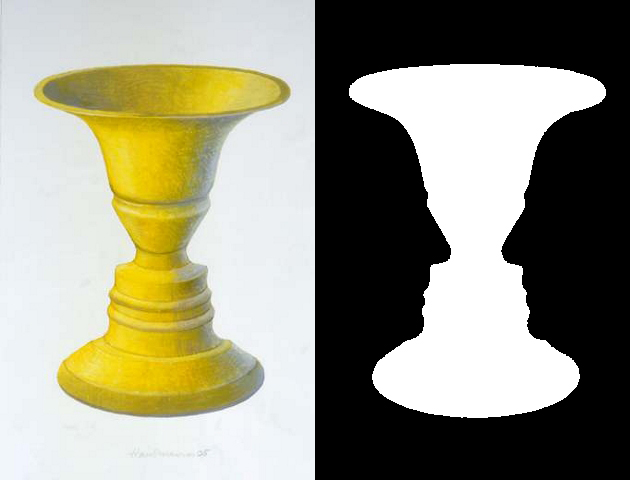
\includegraphics[width=6cm]{rubins_vase.jpg} 
    \caption{Rubins Vase}
  \end{center}
\end{figure}

\subsection{Motivation}
Natural image matting algorithm solves the problem of accurate foreground estimation in an image. As an important and useful technique, it is already widely used in many area like image editing and film production. An effective and accurate matting algorithm can save the manpower cost and improve work efficiency to a large extent. \\

At the same time, with the popularity of smart phones, people take a lot of photos in their daily life, which enhances the demand of image editing. If a matting algorithm can be implemented to run on the mobile device, this feature will very likely to be one of the most important functions of camera.\\ 

Thus, we try to find a matting algorithm which needs user interaction as little as possible and can be run on a mobile device in a reasonable time. \\

\subsection{Related work}
The matting algorihm in ~\cite{Boykov:2001} and ~\cite{Li:2004} translate matting problem into image segmentation problem. By constructing an undirected graph and calculate its minmum cut, it decides whether a pixel belongs to the background or the foreground. Since a fractional alpha will describe the foreground opacity better, the disadvantage of this algorithm is that the alpha it generated is only either 0 or 1. \\

Both of the poisson matting method ~\cite{Sun:2004} and Bayesian matting algorithm ~\cite{Chuang:2001} make use of trimap to perform matting, which labels each pixel as foreground, background, or unknown. Poisson matting method assumes that the matte gradient can be approximated as $\nabla I (F - B)$. However, this assumption is too strong and leads to some local error. \\

The Bayesian matting algorithm perform the most successful matting among the methods described above, which use mixture of oriented Gaussian and then $\alpha, a, b$ are estimated given that distribution. The algorithm performs well when there are little overlap betwen the color distribution on foreground and background, and the unknown area is small. Otherwise it might lead to a erroneous matte as well. \\

In this project, we apply the closed form matting ~\cite{Levin:2006}. The method firstly derives a cost function with color line model, and eliminate $F$ and $B$ from the cost function, leaving $\alpha$ as the only variable. The algorithm calculate the optimal alpha matte that minimizes the cost function. With small amount of user's scribble on natural image as input, high quality $\alpha$ can be generated.

\section{Derivation}
\subsection{Greyscale Image}
In the paper, Levin assumes that foreground image and background image are steady inside small local windows (3 by 3 in his case). Therefore he gives the following mathematical assumption:
$$I_i = \alpha_i F_i + (1 - \alpha_i)B_i$$
$$\Rightarrow \alpha \approx aI_{i} + b, \forall i \in w $$
$$a = \frac{1}{F-B}, b = \frac{-B}{F-B} $$
Levin also defines the cost function $J$ given $\alpha$, a, b. Intuitively, the cost function measures the error of the above approximation of $\alpha$. The bias term $\varepsilon$ is used for numerical stability.
$$J(\alpha, a, b) = \sum_{j \in I}(\sum_{i \in w_j}(\alpha_i - a_jI_i-b_j)^2+\varepsilon a_j^2)$$

The goal of this paper is to find the optimal $(\alpha, a, b)$ to minimize the cost function $J$.\\

\textbf{Theorem1:} Define $J(\alpha)$ as 
$$J(\alpha) = \min_{a,b} J(\alpha, a, b)$$
Then
$$J(\alpha) = \alpha^T L \alpha$$
where $L = \bar{G_k}^T \bar{G_k}$, (i, j)-th entry of $\bar{G_k}$ is:
$$\sum_{k|(i, j) \in w_k}(\delta_{ij} - \frac{1}{|w_k|}(1+\frac{1}{\frac{\varepsilon}{|w_k|} + \sigma_k^2}(I_i - \mu_k)(I_j - \mu_k)))$$
Here $\delta_{ij}$ is the Kronecker delta, $\mu_k$ is the mean of the intensities in the window $w_k$  nearby k, $\sigma_k^2$ is the variance of the intensities in the window $w_k$  nearby k, and $|w_k|$ is the number of pixels in the current window. \\

\textbf{Proof of Theorem1}:\\

Use $G_k$ and $\bar{\alpha_k}$  to denote $J(\alpha)$, where
$$ G_k^T=
  \begin{bmatrix}
    I_1 & I_2 & I_3 & ... & I_{w_k} & \sqrt{\varepsilon}\\
    1 & 1 & 1 & ... & 1 & 0 
  \end{bmatrix} $$
$$ \bar{\alpha_k}^T=
  \begin{bmatrix}
    \alpha_1 & \alpha_2 & \alpha_3 & ... & \alpha_{w_k} & 0 
  \end{bmatrix} $$
$$J(\alpha, a, b) = \sum_{k}||G_k \begin{bmatrix} a_k \\ b_k\end{bmatrix} - \bar{\alpha_k}||^2$$
$$= \sum_k||\begin{bmatrix} I_{1} a_k + b_k \\ I_{2} a_k + b_k \\ \vdots \\ I_{|w_k|} a_k + b_k \\ \sqrt{\varepsilon} a_k \end{bmatrix} - 
\begin{bmatrix}
    \alpha_1 \\ \alpha_2 \\ \alpha_3 \\ \vdots\\ \alpha_{w_k} \\ 0 
\end{bmatrix}||^2$$
$$= \sum_{k}(\sum_{i = 1}^{|w_{k}|}(\alpha_i - a_kI_i-b_k)^2+\varepsilon a_k^2)$$
Meanwhile 
$$J(\alpha, a, b) = \sum_{j \in I}(\sum_{i \in w_j}(\alpha_i - a_jI_i-b_j)^2+\varepsilon a_j^2)$$
Thus
\begin{equation}
J(\alpha, a, b) = \sum_{k}||G_k \begin{bmatrix} a_k \\ b_k\end{bmatrix} - \bar{\alpha_k}||^2
\end{equation}

After rewriting $J(\alpha, a, b)$, for each window, we try to find the $(a_k^*, b_k^*)$ that minimizes $J(\alpha)$, given a specific $\alpha$. Using the solution to the least quares problem we can get:

\begin{equation}
(a_k^*, b_k^*) = argmin||G_k \begin{bmatrix} a_k \\ b_k\end{bmatrix} \bar{\alpha_k}|| = (G_k^TG_k)^{-1}G_k^T \bar{\alpha_k}
\end{equation}

Substituting (3) back to (2), we get:
$$J(\alpha, a, b) = \sum_{k}||G_k \begin{bmatrix} a_k \\ b_k\end{bmatrix} - \bar{\alpha_k}||^2 $$
$$= \sum_{k}||G_k(G_k^TG_k)^{-1}G_k^T \bar{\alpha_k} - \bar{\alpha_k}||^2$$

Let $\bar{G_k} = I - G_k(G_k^T G_k)^{-1}G_k^T$, we get
$$\sum_{k}||G_k(G_k^TG_k)^{-1}G_k^T \bar{\alpha_k} - \bar{\alpha_k}||^2$$
$$ = \sum_{k}|| (I - \bar{G_k})\bar{\alpha_k} - \bar{\alpha_k}||^2 $$
$$ = \sum_{k}|| \bar{G_k}\bar{\alpha_k}||^2 = \sum_{k} (\bar{G_k}\bar{\alpha_k})^T \bar{G_k}\bar{\alpha_k} $$
$$ \sum_{k} \bar{\alpha_k}^T\bar{G_k}^T \bar{G_k}\bar{\alpha_k}$$
Thus we have
$$J(\alpha) = \sum_{k} \bar{\alpha_k}^T\bar{G_k}^T \bar{G_k}\bar{\alpha_k}$$

Then we try to find out the value of $\bar{G_k}$, since $\bar{G_k} = I - G_k(G_k^T G_k)^{-1}G_k^T$, firstly we calculate $G_k^TG_k$: 
$$G_k^TG_k = \begin{bmatrix}
    I_1 & I_2 & I_3 & ... & I_{w_k} & \sqrt{\varepsilon}\\
    1 & 1 & 1 & ... & 1 & 0 
  \end{bmatrix}
  \begin{bmatrix}
    I_1 & 1 \\ I_2 & 1 \\ I_3 & 1 \\ \vdots & \vdots \\ I_{w_k} & 1 \\ \sqrt{\varepsilon} & 0 
  \end{bmatrix} $$
$$ = \begin{bmatrix}
    \sum_{1}^{|w_k|} I_i^2 + \varepsilon & \sum I_i \\
    \sum I_i & |w_k|
  \end{bmatrix}$$

Secondly, with the formula to get the inverse of a 2 by 2 matrix, we can get the inverse of $G_k^TG_k$: 
$$(G_k^TG_k)^{-1} = \frac{\begin{bmatrix}
    |w_k| & \sum -I_i \\
    \sum -I_i & \sum_{1}^{|w_k|} I_i^2 + \varepsilon
  \end{bmatrix}}{|w_k|(\sum I_i^2 + \varepsilon) - (\sum I_i)^2} 
  $$

Thirdly, we calcualte the $G_k(G_k^TG_k)^{-1}$:

$$G_k(G_k^TG_k)^{-1} = \frac{\begin{bmatrix}
    I_1 & 1 \\ I_2 & 1 \\ \vdots & \vdots \\ I_{w_k} & 1 \\ \sqrt{\varepsilon} & 0 
  \end{bmatrix} 
  \begin{bmatrix}
    |w_k| & \sum -I_i \\
    \sum -I_i & \sum I_i^2 + \varepsilon
  \end{bmatrix}}{|w_k|(\sum I_i^2 + \varepsilon) - (\sum I_i)^2} $$
$$ = \frac{\begin{bmatrix}
    I_1w_k - \sum I_i & -I_1 \sum I_i + \sum I_i^2 + \varepsilon \\
    I_2w_k - \sum I_i & -I_2 \sum I_i + \sum I_i^2 + \varepsilon \\
    \hdots & \hdots \\
    I_{|w_k|}w_k - \sum I_i & -I_{|w_k|} \sum I_i + \sum I_i^2 + \varepsilon \\
    \sqrt{\varepsilon}|w_k| & -\sqrt{\varepsilon}\sum I_i
  \end{bmatrix}}{|w_k|(\sum I_i^2 + \varepsilon) - \sum I_i^2}$$\\
Fourthly, we calcualte $G_k(G_k^TG_k)^{-1}G_k^T $:
$$G_k(G_k^TG_k)^{-1}G_k^T = G_k(G_k^TG_k)^{-1}
  \begin{bmatrix}
    I_1 & I_2 & ... & I_{w_k} & \sqrt{\varepsilon}\\
    1 & 1 & ... & 1 & 0 
  \end{bmatrix} $$

When $i \le p, j \le q$, we have 
$$[G_k(G_k^TG_k)^{-1}G_k^T]_{i, j} $$
$$ \frac{(I_i |w_k| - \sum I_i) * I_j - I_i \sum I_i + \sum I_i^2 + \varepsilon}{|w_k|(\sum_{1}^{|w_k|} I_i^2 + \varepsilon) - (\sum I_i)^2}$$
$$= \frac{I_i I_j |w_k| - (I_j + I_i)\sum I_i + \sum I_i^2 + \varepsilon}{|w_k|(\sum_{1}^{|w_k|} I_i^2 + \varepsilon) - (\sum I_i)^2}$$

Since $\mu_k$ and $\sigma_k^2$ are the mean and the variance of the intensities in the window $w_k$  nearby k, we have:
$$\mu_k = \frac{1}{|w_k|}\sum I_i \Rightarrow \sum I_i = |w_k|\mu_k$$
$$\sigma_k^2 = E(x^2) - E(x)^2 = \frac{1}{|w_k|}\sum I_i^2 - \mu_k^2 $$
$$\Rightarrow \sum I_i^2 = (\sigma_k^2 + \mu_k^2)|w_k|$$

Substituting the $\sum I_i^2$ and $\sum I_i$ with $\mu_k$ and $\sigma_k^2$, we get
$[G_k(G_k^TG_k)^{-1}G_k^T]_{i, j}$
$$= \frac{I_i I_j |w_k| - (I_j + I_i)|w_k|\mu_k + (\sigma_k^2 + \mu_k^2)|w_k| + \varepsilon}{(\sigma_k^2 + \mu_k^2)|w_k|^2 + \varepsilon|w_k| - |w_k|^2\mu_k^2} $$
$$ = \frac{I_i I_j |w_k| - (I_j + I_i)|w_k|\mu_k + |w_k|\mu_k^2 + |w_k|\sigma_k^2 + \varepsilon}{\sigma_k^2|w_k|^2 + \varepsilon|w_k|}$$
$$ = \frac{I_i I_j - (I_j + I_i)\mu_k + \mu_k^2}{\sigma_k^2|w_k| + \varepsilon} + 
\frac{|w_k|\sigma_k^2 + \varepsilon}{\sigma_k^2|w_k|^2 + \varepsilon|w_k|}$$
$$ = \frac{1}{|w_k|}(1 + \frac{I_i I_j - (I_j + I_i)\mu_k + \mu_k^2}{\sigma_k^2 + \frac{\varepsilon}{|w_k|}})$$
$$= \frac{1}{|w_k|}(1 + \frac{(I_i - \mu_k)(I_j - \mu_k)}{\sigma_k^2 + \frac{\varepsilon}{|w_k|}})$$
$$= \frac{1}{|w_k|}(1 + \frac{1}{\frac{\varepsilon}{|w_k|} + \sigma_k^2}(I_i - \mu_k)(I_j - \mu_k))$$

Since $\bar{G_k} = I - G_k(G_k^TG_k)^{-1}G_k^T$, we have:
$$[\bar{G_k}]_{i,j} = [I - G_k(G_k^TG_k)^{-1}G_k^T]_{i,j} $$
$$= [I]_{i,j} - [G_k(G_k^TG_k)^{-1}G_k^T]_{i,j}$$
$$= \delta_{ij} - \frac{1}{|w_k|}(1 + \frac{1}{\frac{\varepsilon}{|w_k|} + \sigma_k^2}(I_i - \mu_k)(I_j - \mu_k))$$

Therefore, we can denote $J(\alpha) = \alpha^T L \alpha$, where $L = \bar{G_k}^T\bar{G_k}$ and 
$$[\bar{G_k}]_{i,j} = \delta_{ij} - \frac{1}{|w_k|}(1 + \frac{1}{\frac{\varepsilon}{|w_k|} + \sigma_k^2}(I_i - \mu_k)(I_j - \mu_k))$$

\subsection{Color Image}

To prove that $J(\alpha)$ applies to the color images as well, Levin uses color line model ~\cite{Omer:2004} to represent the color image. \\

Color line model assumes that the foreground color and the background color inside a small window is an interpolation of two color points, i.e.,
\begin{equation}
F_i = \beta^F_{i} F_1 + (1-\beta^F_{i})F_2
\end{equation}
\begin{equation}
B_i = \beta^B_{i} B_1 + (1-\beta^B_{i})B_2
\end{equation}

Where $\beta_i$ is a constant factor. $F_1$, $B_1$ and $F_2$, $B_2$ are the foreground color and background color of two different points.\\

Using color line model, Levin claims that αi can be represented as:
$$\alpha_i = \sum_{c}a^cI_i^c + b, \forall i \in w$$

\textbf{Proof:} \\
Substitude (4) and (5) into $I_i^c = \alpha_i F_i^c + (1-\alpha_i)B_i^c$:
$$\Rightarrow I_i^c = \alpha_i (\beta^F_{i} F_1^c + (1-\beta^F_{i})F_2^c)$$
$$ + (1-\alpha_i)(\beta^B_{i} B_1^c + (1-\beta^B_{i})B_2^c)$$
$$\Rightarrow I_i^c - B_2^c = \alpha_i (\beta^F_{i} F_1^c + (1-\beta^F_{i})F_2^c)$$
$$ + (1-\alpha_i)(\beta^B_{i} B_1^c + (1-\beta^B_{i})B_2^c) - B_2^c$$
$$ = (F_2^c - B_2^c)\alpha_i + (F_1^c - F_2^c)\alpha_i \beta_i^F + (B_1^c - B_2^c)(1-\alpha_i)$$
$$ = \begin{bmatrix}
    F_2^c - B_2^c & F_1^c - F_2^c & B_1^c - B_2^c
  \end{bmatrix}
  \begin{bmatrix}
    \alpha_i \\ \alpha_i \beta_i^F \\ (1-\alpha_i)\beta_i^B
  \end{bmatrix} $$
Let $$H = \begin{bmatrix}
    F_2^R - B_2^R & F_1^R - F_2^R & B_1^R - B_2^R \\
    F_2^G - B_2^G & F_1^G - F_2^G & B_1^G - B_2^G \\
    F_2^B - B_2^B & F_1^B - F_2^B & B_1^B - B_2^B 
  \end{bmatrix}$$
Then from above we know:
$$H\begin{bmatrix}
    \alpha_i \\ \alpha_i \beta_i^F \\ (1-\alpha_i)\beta_i^B
  \end{bmatrix} = 
  \begin{bmatrix}
    I_i^R \\ I_i^G \\ I_i^B
  \end{bmatrix} - 
  \begin{bmatrix}
    B_2^R \\ B_2^G \\ B_2^B
  \end{bmatrix}$$
$$\Rightarrow \begin{bmatrix}
    \alpha_i \\ \alpha_i \beta_i^F \\ (1-\alpha_i)\beta_i^B
  \end{bmatrix} = H^{-1}(
  \begin{bmatrix}
    I_i^R \\ I_i^G \\ I_i^B
  \end{bmatrix} - 
  \begin{bmatrix}
    B_2^R \\ B_2^G \\ B_2^B
  \end{bmatrix})$$

Denote $\begin{bmatrix} a^R & a^G & a^B \end{bmatrix}$ as the first row of $H^{-1}$, then we obtain: 
$$\alpha_i = 
(a^RI_i^R + a^GI_i^G + a^BI_i^B)-(a^RB_2^R + a^GB_2^G + a^BB_2^B)$$

Let $b = a^RB_2^R + a^GB_2^G + a^BB_2^B$, we obtain:
$$\alpha_i = \sum_{c}a^cI_i^c + b, \forall i \in w$$

By which we can also derive $J(\alpha) = \alpha^T L \alpha$ using the similar derivation in section 2.1. \\

Similar to the cost function of gray­scale images, Levin defines the cost function as:
$$J(\alpha, a, b) = \sum_{j \in I}(\sum_{i \in w_j}(\alpha_i - \sum_c a_j^c I_i^c-b_j)^2+\varepsilon \sum_{c}{a_j^c}^2)$$

Using the similar derivation process in section 2.1, we can eliminate a and b in the above equation and get $J(\alpha) = \alpha^T L \alpha$ where $L = \bar{G_k}^T \bar{G_k}$ and (i, j)-th element of $\bar{G_k}$ is:
$$\sum_{k|(i,j) \in w_k} (\delta_{ij} - \frac{1}{|w_k|}(1 + (I_i - \mu_k)(\sum_k + \frac{\varepsilon}{|w_k|}I_3)^{-1}(I_j - \mu_k)))$$

where $\sum_k$ is a convariance matrix.
\subsection{User Constraint}
As mentioned in the introduction, user constrained is required to obtain a meaningful alpha matte. We allow users to indicate some background pixels($\alpha = 0$) and some foreground pixels($\alpha = 1$). With S as the user constraint, we solve for:
$$\alpha = argmin(\alpha^T L \alpha), s.t.\alpha_i = s_i, \forall i \in S $$

\subsection{Alpha Derivation}
The target of image matting is to find the pixel’s foreground opacity $\alpha$, which can be derived by solution the equation:
$$\alpha = argmin(\alpha^T L \alpha), s.t.\alpha_i = s_i, \forall i \in S $$

The value of $J(\alpha)$ will be minimal when the derivative of $J(\alpha)$ is 0, thus we have:
$$\frac{\partial J(\alpha)}{\partial \alpha} = 0$$
$$\Rightarrow \frac{\partial{(\alpha^T L \alpha)}}{\partial \alpha} = 2L\alpha$$
$$\Rightarrow L\alpha = 0$$

Denote $const\_map$ as the matrix which is N by 1, whose value is 1 on the scribbled pixel and 0 otherwise. Denote $const\_value$ as the matrix which is N by 1, which is derived from $const\_map .* image(:)$. It is obvious that:
$$const\_map * \alpha = const\_val$$

Combining the forumlas above together and we get
$$(L + \lambda * const\_map)\alpha = \lambda * const\_val$$
Where $\lambda$ is a heuristic value to make a balance between the user constraint and the smoothness of the image.\\

Since both $L + \lambda * const\_map$ and $\lambda * const\_val$ can be calculated from image data, the only unknown variable is $\alpha$. Thus by solving this equation we can get value of $\alpha$.

% \begin{figure*}[h]
% \begin{center}
% \begin{tikzpicture}[node distance=2cm,auto,>=latex']
%   \node [coordinate] (start) {};
%   \node [obj, below of = start, node distance=1.5cm] (imageReader) {ImageReader};
%   \node [obj, below of = imageReader] (mattingPerformer) {MattingPerformer};
%   \node [obj, below of  = mattingPerformer] (imagePrinter) {ImagePrinter};
%   \node [coordinate, below of = imagePrinter, node distance=1.5cm] (end){};
%   \node [obj, right of = mattingPerformer, node distance=5.5cm] (alphaCalculator) {AlphaCalculator};
%   \node [obj, above right of = alphaCalculator, node distance=3cm] (laplacianCalculator) {LaplacianCalculator};
%   \node [obj, below right of = alphaCalculator, node distance=3cm] (sparseMatrixEquationSolver) {SparseMatrixEquationSolver};

%   \path[->] (start) edge node {File path} (imageReader);
%   \path[->] (imageReader) edge node {Image matrix} (mattingPerformer);
%   \path[->] (alphaCalculator) edge node {Image matrix} (laplacianCalculator);
%   \path[->] (laplacianCalculator) edge node {Laplacian matrix} (alphaCalculator);
%   \path[->] (alphaCalculator) edge node {sparse matrix A, vector B} (sparseMatrixEquationSolver);
%   \path[->] (sparseMatrixEquationSolver) edge node {x = $A \backslash B$ } (alphaCalculator);
%   \path[->] (mattingPerformer) edge node {Image matrix} (alphaCalculator);
%   \path[->] (alphaCalculator) edge node {alpha} (mattingPerformer);
%   \path[->] (mattingPerformer) edge node {Matting image matrix} (imagePrinter);
%   \path[->] (imagePrinter) edge node {Window shows result} (end);
% \end{tikzpicture}
% \caption{Matting pipeline}
% \end{center}
% \end{figure*}

\section{Implementation}
We implement the matting algorithm in an OOP programming style. The pipeline of the algorithm is shown in Figure 1. \\

Firstly, ImageReader is given the file paths of original image and scribbled image. Then it send image matrices to the MattingPerformer. \\

Secondly, MattingPerformer gives image matrix to AlphaCalculator. With the help from LaplacianCalculator and SparseMatrixEquationSolver, the AlphaCalculator gets the alpha is return it to the MattingPerformer. Then MattingPerformer performs alpha on the imagel, generates matting image and returns image to the ImagePrinter.\\

Finally, ImagePrinter receives the matrix of matting image. It create a canvas and draw the image on it to show the matting result. 

\subsection{ImageReader}
Given the file path of the image, ImageReader will read the image and return a matrix to represent the image. The function readImage() use OpenCV to read image data and write into a matrix. 

In our implementation, we use ImageReader to read two images: the original image and the original image with user input. The pixels of value 1 in the image represent foreground while the pixels of value 0 prepresent background. 

\subsection{LaplacianCalculator}
In the section 2, we proved that $J(\alpha) = \alpha^T L \alpha$, where L is an N by N matrix whose (i, j)-th element is:
$$\sum_{k|(i,j) \in w_k} (\delta_{ij} - \frac{1}{|w_k|}(1 + (I_i - \mu_k)(\sum_k + \frac{\varepsilon}{|w_k|}I_3)^{-1}(I_j - \mu_k)))$$

Given the matrices of image and scribbled image. The task of the LaplacianCalculator is to get such a matrix L. 

\subsection{SparseMatrixEquationSolver}
SparseMatrixEquationSolver is specially used to solve the equation $Ax=B$, where A is a sparse matrix of N by N and N is the pixel number of an image. \\

Assume an image of 400 by 300 pixels, the number of pixel will be 120,000. And the size of matrix A will be 120,000 by 120,000. To store such a large matrix, we use the sparse matrix library, which is provided by Eigen. Then we use umfpack of suitesparse library to solve the equation of $Ax=B$. \\

\subsection{AlphaCalculator}
Alpha calculator will firstly use LaplacianCalculator to get laplacian matrix. Then form the sparse matrix equation and use SparseMatrixEquationSolver to solve it and get alpha values.

\subsection{MattingPerformer}
Matting performer uses AlphaCalculator to get alpha of image. Then apply alpha on image and get matting image.

\subsection{ImagePrinter}
ImagePrinter receieves the result from MattingPerformer and then print the matting result. The function writeImage use OpenCV to create window and draw matrix of image on it. 

\newpage
\section{Experimental results}
When we have obtained the foreground opacity $\alpha$, we apply $\alpha$ on the input image. We use following formula to get foreground image and backround image:
$$I_{foreground} = I * \alpha$$
$$I_{background} = I * (1-\alpha)$$

Figure 2, 3, 4 shows the matting results for different input image. The first image (a) in each figure is the original input image. The second image (b) is the input image with scribble provided by user interaction, where 0 means the pixel belongs to the background and 1 means the pixel belongs to the foreground. The third image is the foreground image of matting result $I_{foreground}$ and the fourth image is the background image of matting result $I_{background}$.\\

From these figure we can find that, with proer user input, the matting algorithm can successfully separate a foreground object from the background. Some fine or fuzzy features, like the hair of the kid in the Figure 2. the featherlike hairs of dandelion in Figure 3, and the feather of peacock in Figure 4. \\

\begin{figure}[h!]
  \centering
  \begin{subfigure}{0.24\textwidth}
    \centering
    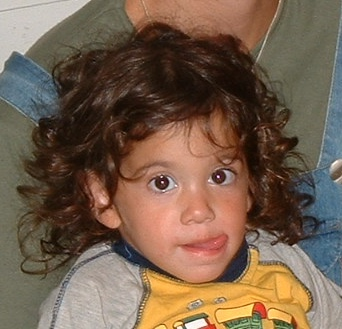
\includegraphics[width=4cm]{./result/kid/kid.jpg}
    \caption{}
  \end{subfigure}
  \begin{subfigure}{0.24\textwidth}
    \centering
    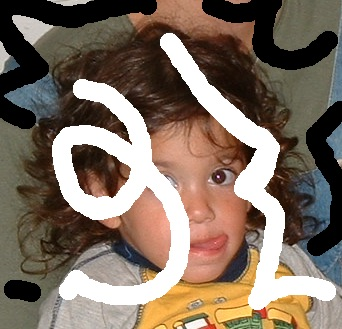
\includegraphics[width=4cm]{./result/kid/kid_m.jpg}
    \caption{}
  \end{subfigure}
  \begin{subfigure}{0.24\textwidth}
    \centering
    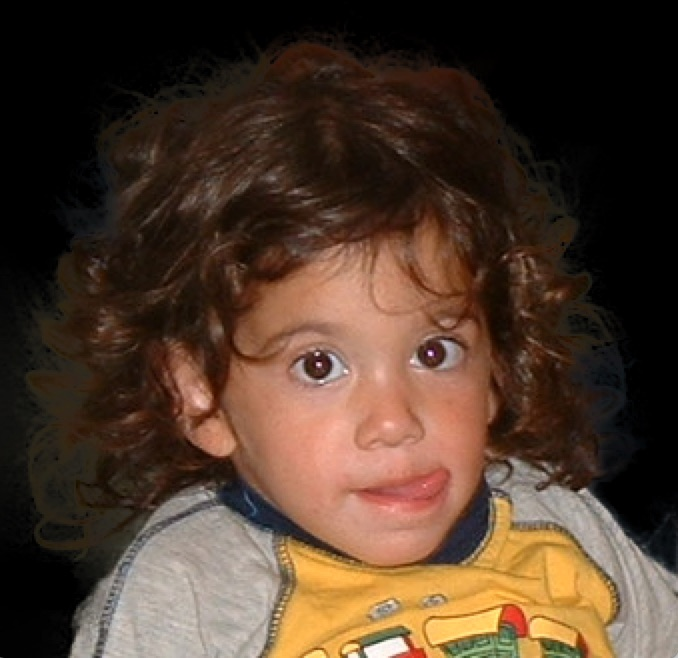
\includegraphics[width=4cm]{./result/kid/kid_foreground.jpg}
    \caption{}
  \end{subfigure}
  \begin{subfigure}{0.24\textwidth}
    \centering
    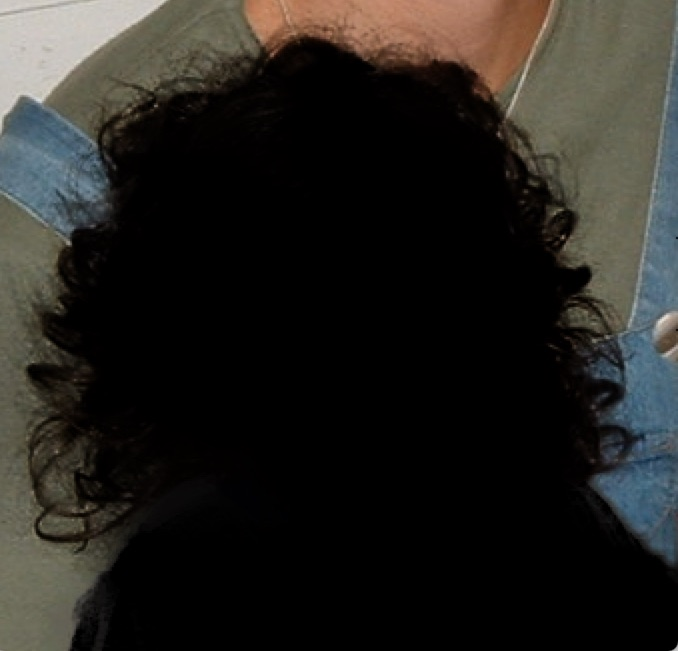
\includegraphics[width=4cm]{./result/kid/kid_background.jpg}
    \caption{}
  \end{subfigure}    
  \caption {Matting result for kid.jpg}
\end{figure}

\begin{figure}[h!]
  \centering
  \begin{subfigure}{0.24\textwidth}
    \centering
    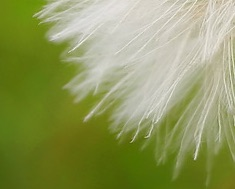
\includegraphics[width=4cm]{./result/dandelion/dandelion.jpg}
    \caption{}
  \end{subfigure}
  \begin{subfigure}{0.24\textwidth}
    \centering
    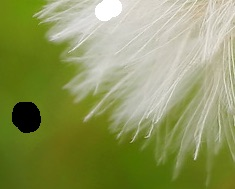
\includegraphics[width=4cm]{./result/dandelion/dandelion_m.jpg}
    \caption{}
  \end{subfigure}
  \begin{subfigure}{0.24\textwidth}
    \centering
    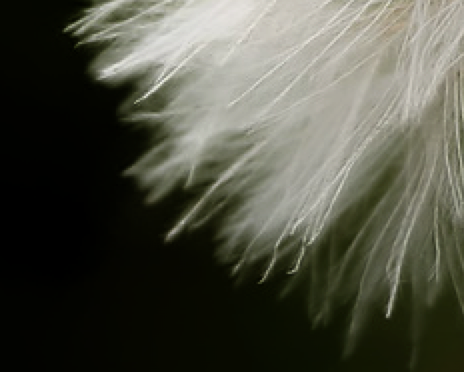
\includegraphics[width=4cm]{./result/dandelion/dandelion_foreground.png}
    \caption{}
  \end{subfigure}
  \begin{subfigure}{0.24\textwidth}
    \centering
    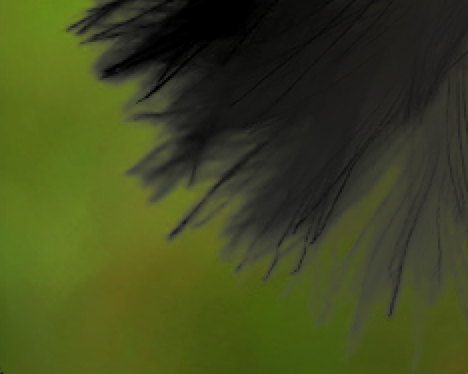
\includegraphics[width=4cm]{./result/dandelion/dandelion_background.png}
    \caption{}
  \end{subfigure}    
  \caption {Matting result for dandelion.jpg}
\end{figure}

\begin{figure}[h!]
  \centering
  \begin{subfigure}{0.24\textwidth}
    \centering
    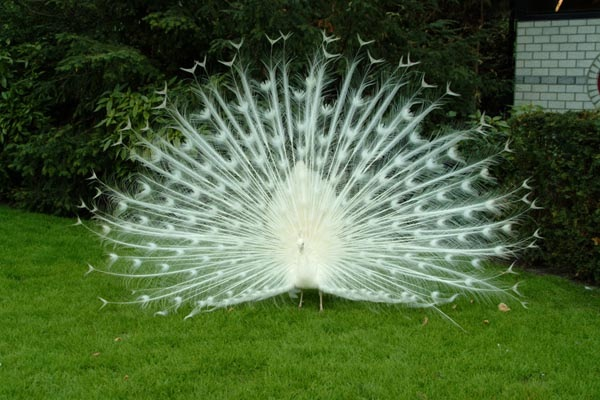
\includegraphics[width=4cm]{./result/peacock/peacock.jpg}
    \caption{}
  \end{subfigure}
  \begin{subfigure}{0.24\textwidth}
    \centering
    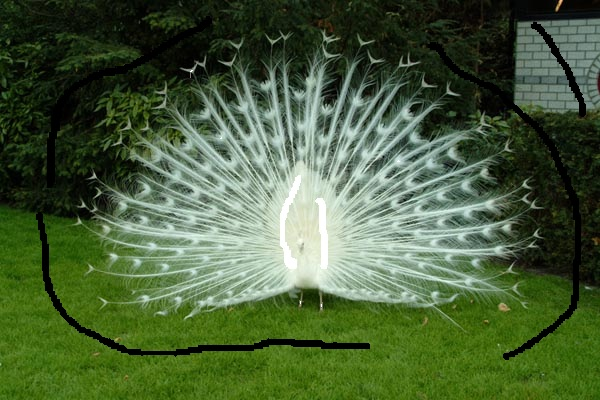
\includegraphics[width=4cm]{./result/peacock/peacock_m.jpg}
    \caption{}
  \end{subfigure}
  \begin{subfigure}{0.24\textwidth}
    \centering
    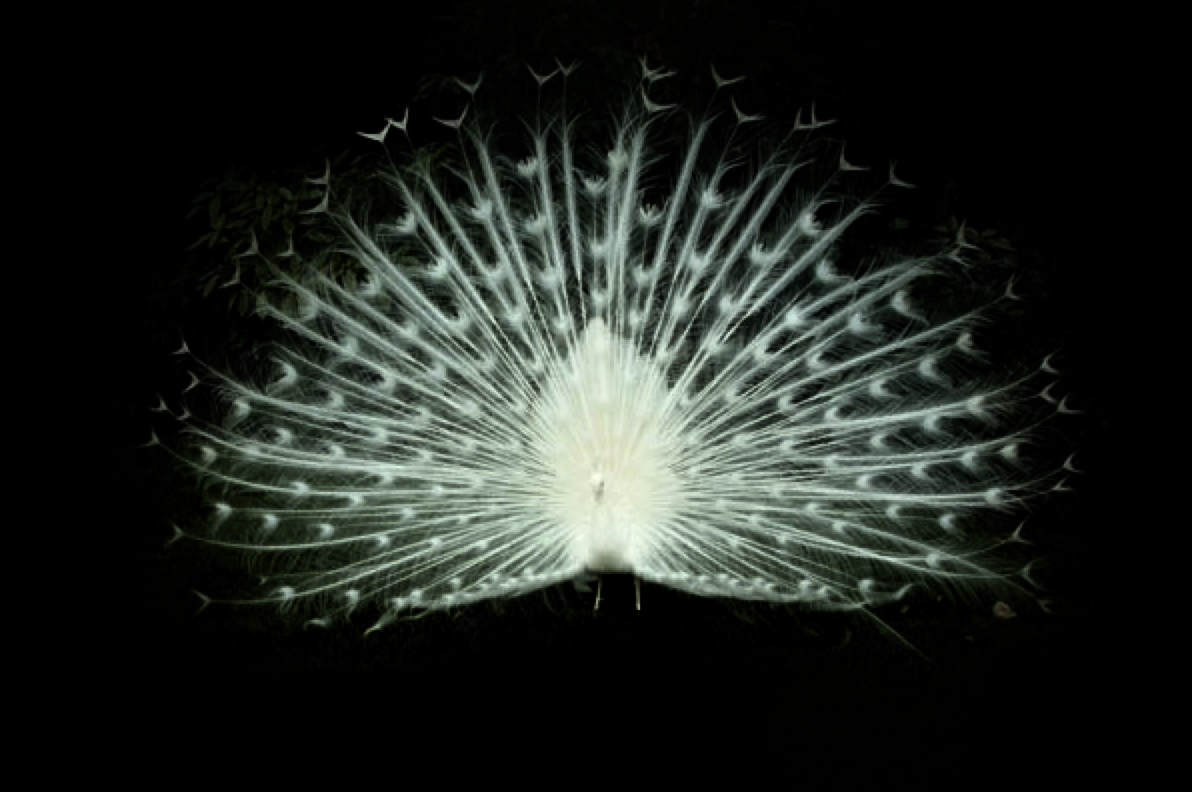
\includegraphics[width=4cm]{./result/peacock/peacock_foreground.png}
    \caption{}
  \end{subfigure}
  \begin{subfigure}{0.24\textwidth}
    \centering
    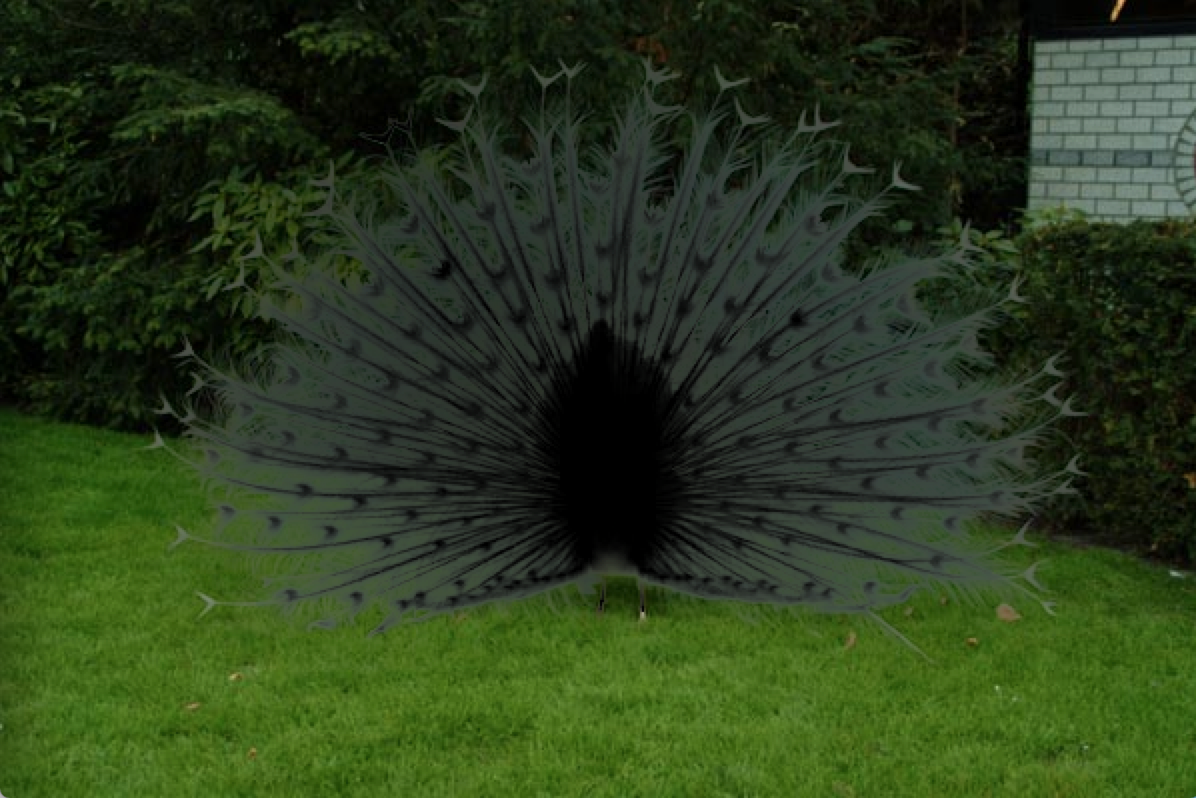
\includegraphics[width=4cm]{./result/peacock/peacock_background.png}
    \caption{}
  \end{subfigure}    
  \caption {Matting result for peacock.jpg}
\end{figure}

\newpage

\section{Conclusion}
The matting algorithm described in the this project can perform image matting properly. However, during the implementation, we find the time complexity is actually quite large. \\

\section{Future work}
We can use eigen value of Laplacian matrix. \\

\bibliography{project}
\bibliographystyle{acl2012}

\end{document}